% Copyright (C) 2011 Thomas L. Kula
% All Rights Reserved
%
% See the file LICENSE for license terms.
\documentclass[12pt]{article}
\usepackage{graphicx}
\usepackage{rotating}
\usepackage{fix-cm}
\usepackage{multirow}
\setlength{\paperwidth}{5.5in}
\setlength{\paperheight}{8.5in}
\setlength{\textheight}{7.45in}
\setlength{\topmargin}{-1.0in}
\setlength{\oddsidemargin}{-0.5in}
\setlength{\evensidemargin}{-0.5in}
\setlength{\textwidth}{4.0in}
\setlength{\parindent}{0in}
\setlength{\parskip}{3mm}
\usepackage[print]{booklet} \nofiles
\source{\magstep0}{5.5in}{8.5in}
\target{\magstep0}{11in}{8.5in}
\setpdftargetpages
\pagestyle{empty}
\begin{document}


\begin{center}
{\fontsize{36}{48}\selectfont \textsc{Haiku a Day }}
\end{center}

\vspace*{3.5cm}

{\fontsize{20}{40}\selectfont 


Why the laundromat?

I get more work done there

Than I do elsewhere.

}

\vspace*{5.0cm}
\begin{center}
{\large{Issue 68: February 2011}} \\[5mm]
{\fontsize{8}{8}\selectfont  \textsc{ St. Joshua Norton Press }} \\[1mm]
{\fontsize{6}{6}\selectfont Mathom House in Midtown \textbar The People's Republic of Ames }
\end{center}


\newpage

Brief tautings of mid 40 degree F weather mixed with cold and
snow. Spring is such a tease.

--- Thomas

http://kula.tproa.net/had/ \\
kula@tproa.net

Download this and previous HADs at the website, so you can
print out your own (DIY, yeah!) or if you want me to send
you one, send me your address, and maybe a stamp if you
are feeling nice. Or send me something you've made ---
trades always appreciated, postcards are nice too.

\vfill

\newpage

1 February 2011

City reflecting \\
Sodium orange in the snow \\
Warm glow in cold skies

2 February 2011

Whiny singing drones \\
As I pass a house walking \\
I quicken my pace

3 February 2011

A pathetic beach \\
Sand grains on the welcome mat \\
Grate, do not relax

4 February 2011

Refraining refrains \\
Render rhymes ridiculous \\
Really required

5 February 2011

Seeking salvation \\
Some squander serenity \\
Some society

6 February 2011

This theme thoroughly \\
Transcends the taste thoughtfulness \\
Therefore, this time: halt

7 February 2011

Fibonacci scribes \\
A series ever closer \\
Golden ratio


\newpage

8 February 2011

Originator \\
The birthplace of lies hidden \\
Unsuspectingly

9 February 2011

Goofy Kroger rice \\
Nearly all done, some still raw \\
How does that happen?

10 February 2011

Leftovers combine \\
A strange ad-hoc mixing dish \\
Turns out pretty good

11 February 2011

You're ever so vain. \\
Probably think this haiku's \\
About you, don't you?

12 February 2011

Gallons of Chili \\
I just wanted to test it \\
But did it in full

13 February 2011

Chopping out the waste \\
One's waste, another's treasure \\
Makes things difficult

14 February 2011

Early Spring preview \\
A strong urge to shed jackets \\
Looking for tree buds


\newpage


15 February 2011

Visualize calm \\
Let your mind empty as a \\
Leaf floats on the wind

16 February 2011

Repository \\
That's taking so long to clone \\
I am impatient

17 February 2011

Day after dinner \\
I'm still full around lunch time \\
Really ate too much

18 February 2011

Cold dread, panicing \\
A stupid mistake, coursing \\
Chilling all my blood

19 February 2011

A job done early \\
Makes me spend Saturday night \\
At work, not Sunday

20 February 2011

The campaign for spring \\
Sweet flowers, ideas planted \\
Struggling to bloom

21 February 2011

Barnacles of snow \\
Crusted on automobiles \\
Winter's last hurrah


\newpage

22 February 2011

Itch unscratchable \\
An insolence maddening \\
Small nit magnified

23 February 2011

Now wasting my time \\
Learning nothing new, sleepy, \\
I yearn for coffee

24 February 2011

Jargon's fake patois \\
Rendering unreadable \\
Things I will ignore

25 February 2011

Fire seducing \\
Rapt attention, indoor coals \\
Window keeps alive

26 February 2011

Acres of clothing \\
Endless yards to look through \\
To find just one thing

27 February 2011

End-of-month pizza \\
The conjection of gumption \\
And few groceries

28 February 2011

Dominated by slush \\
A helpful sign, spring awakens? \\
Will it be here soon?



\newpage

\begin{center}
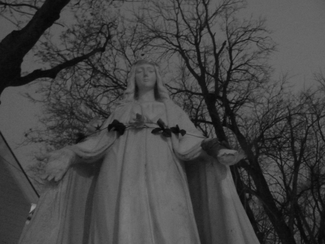
\includegraphics{mary-snow.png}

Winter gives one more hurrah \\
{\tt kula.tproa.net/photos/2011/20110201-snow/ }
\end{center}



\newpage

\thispagestyle{empty}
\vspace*{12cm}
\begin{sideways}
\Large{St. Joshua Norton Press}
\end{sideways}
\begin{sideways}
\Large{PO Box 980461}
\end{sideways}
\begin{sideways}
\Large{Ypsilanti MI 48198}
\end{sideways}


\end{document}


